% preamble and style file for M&R lecture slides
\documentclass[11.5pt,sans,english]{beamer}

\usetheme{EastLansing}
\usecolortheme{lily}

\usepackage[most]{tcolorbox}

\usepackage{verbatim}
%\usepackage{ulem}
%\usepackage{fontawesome}
%\usepackage{tikz}
%\usepackage{pifont}
%\usepackage{tabularx}
\usepackage{array,booktabs,xcolor,colortbl,multirow,rotating,amssymb}
%\usepackage{amsmath}
% \usepackage{vwcol}
% \usepackage[T1]{fontenc}

  
\newcommand\vect[1]{\underline{\mathbf{#1}}}
\newcommand\unitvect[1]{\hat{\boldsymbol{#1}}}
%\newcommand\hatdot[1] { \hat{ \dot{ \boldsymbol{#1} } } }

\newtcbox
{\keyc}{on line,arc=2pt, colback=yellow!30!white, colframe=yellow!30!black, before upper={\rule[-3pt]{0pt}{10pt} },boxrule=1pt,boxsep=0pt,left=6pt,right=6pt,top=2pt,bottom=2pt,}

\newtcbox
{\keyb}{on line,arc=1pt, colback=blue!30!white, colframe=blue!30!black, before upper={\rule[-3pt]{0pt}{10pt} },boxrule=1pt,boxsep=0pt,left=6pt,right=6pt,top=2pt,bottom=2pt,}

\newtcbox
{\keyl}{on line,arc=1pt, colback=pink!30!white, colframe=blue!30!black, before upper={\rule[-3pt]{0pt}{10pt} },boxrule=1pt,boxsep=0pt,left=6pt,right=6pt,top=2pt,bottom=2pt,}

\newtcbox
{\keyw}{on line,arc=1pt, colback=red!30!white, colframe=blue!30!black, before upper={\rule[-3pt]{0pt}{10pt} },boxrule=1pt,boxsep=0pt,left=6pt,right=6pt,top=2pt,bottom=2pt,}

\newtcbox
{\keya}{on line,arc=1pt, colback=purple!30!white, colframe=blue!30!black, before upper={\rule[-3pt]{0pt}{10pt} },boxrule=1pt,boxsep=0pt,left=6pt,right=6pt,top=2pt,bottom=2pt,}

\newtcbox[auto counter,number within=section]
{keyf}
{
enhanced,
on line,
  boxsep=0pt,
  left=6pt,right=6pt,top=2pt,bottom=2pt,
  arc=5pt,
  boxrule=1pt,
  rightrule=38pt,
colback=green!10!white, 
colframe=green!50!black, 
title=\thetcbcounter,
detach title,
overlay unbroken and first ={
    \node[%rotate=90,
          %minimum width=1cm,
          anchor=south,
          font=\sffamily\bfseries\tiny,
          %yshift=-10pt,
          yshift=-5pt,
          xshift=-20pt,
          white]
    at (frame.east) {\thetcbcounter};
  }
}


\usepackage{xcolor}

%\usepackage{hyperref}
%\hypersetup{
%  pdfauthor={Lily Asquith},
%  urlcolor=blue,
%  colorlinks=true,
%  linkcolor=blue,
%  bookmarks=true
%}

%---------------------------------------------%
%              LILY'S COLOURS           %
%---------------------------------------------%
\definecolor{Wash}{RGB}{204,204,204}
%\definecolor{Pinky}{RGB}{254,200,254}%violet
\definecolor{Pinky}{RGB}{219,	240,	253}%violet
\definecolor{Bluey}{RGB}{0,190,255}%deep sky blue
\definecolor{DarkGrey}{RGB}{28,66,137}%dar grey
\definecolor{SussexWhite}{RGB}{253,255,254}%dar grey
\definecolor{LightGray}{RGB}{184,184,255}
\definecolor{YesGreen}{RGB}{0,128,0}
\definecolor{NoRed}{RGB}{250,0,0}



\definecolor{myred}{RGB}{255,153,153}
\definecolor{myorange}{RGB}{255,204,153}
\definecolor{myyellow}{RGB}{255,255,153}
\definecolor{mygreen}{RGB}{153,255,153}
\definecolor{mycyan}{RGB}{153,255,255}
\definecolor{myblue}{RGB}{153,204,255}
\definecolor{myviolet}{RGB}{153,153,255}
\definecolor{mypurple}{RGB}{204,153,255}
\definecolor{mypink}{RGB}{255,204,255}
\definecolor{mycoral}{RGB}{255,153,204}

%-----------------------------------------------------%
%              LILY'S COLUMN TYPES          %
%-----------------------------------------------------%
\newcolumntype{a}{>{\raggedright\arraybackslash}l}	
\newcolumntype{q}{>{\raggedright\arraybackslash}m{8cm}} 

%--------------------------------------------%
%              LILY'S SYMBOLS          %
%--------------------------------------------%
\newcommand{\dfinger}{\large{\textcolor{black}{\ding{43}}}\scriptsize}
\newcommand{\dstar}{\large{\textcolor{black}{\ding{76}}}\scriptsize}
\newcommand{\dwrite}{\large{\textcolor{black}{\ding{45}}}\scriptsize}
\newcommand{\ddiamond}{\small{\textcolor{DarkGrey}{\ding{117}}}\scriptsize}
\newcommand{\ddiamondwhite}{\small{\textcolor{SussexWhite}{\ding{117}}}\scriptsize}
\newcommand{\experiment}{\small{\textcolor{magenta}{\faCogs }}\scriptsize}
\newcommand{\watchit}{\textcolor{blue}{ \faYoutube}}


\makeatletter
\newcommand\notsotiny{\@setfontsize\notsotiny{6.5}{7.5}}
\makeatother


% 
\title[ Mechanics \& Relativity]{Mechanics \& Relativity}
%\subtitle{\textbf{Topic 1: Kinematics }}
\author[Dr Lily Asquith (Lily)]{ Dr Lily Asquith (Lily)}
\date[Week 3]{Week 3}
\logo{

\includegraphics[width=1.5cm]{../../utils/uslogo.jpg}
}


\begin{document}


\begin{frame}
\titlepage
\end{frame} 


\begin{frame}
\frametitle{Submit your workshop problem (vectors) for marking by noon Friday}
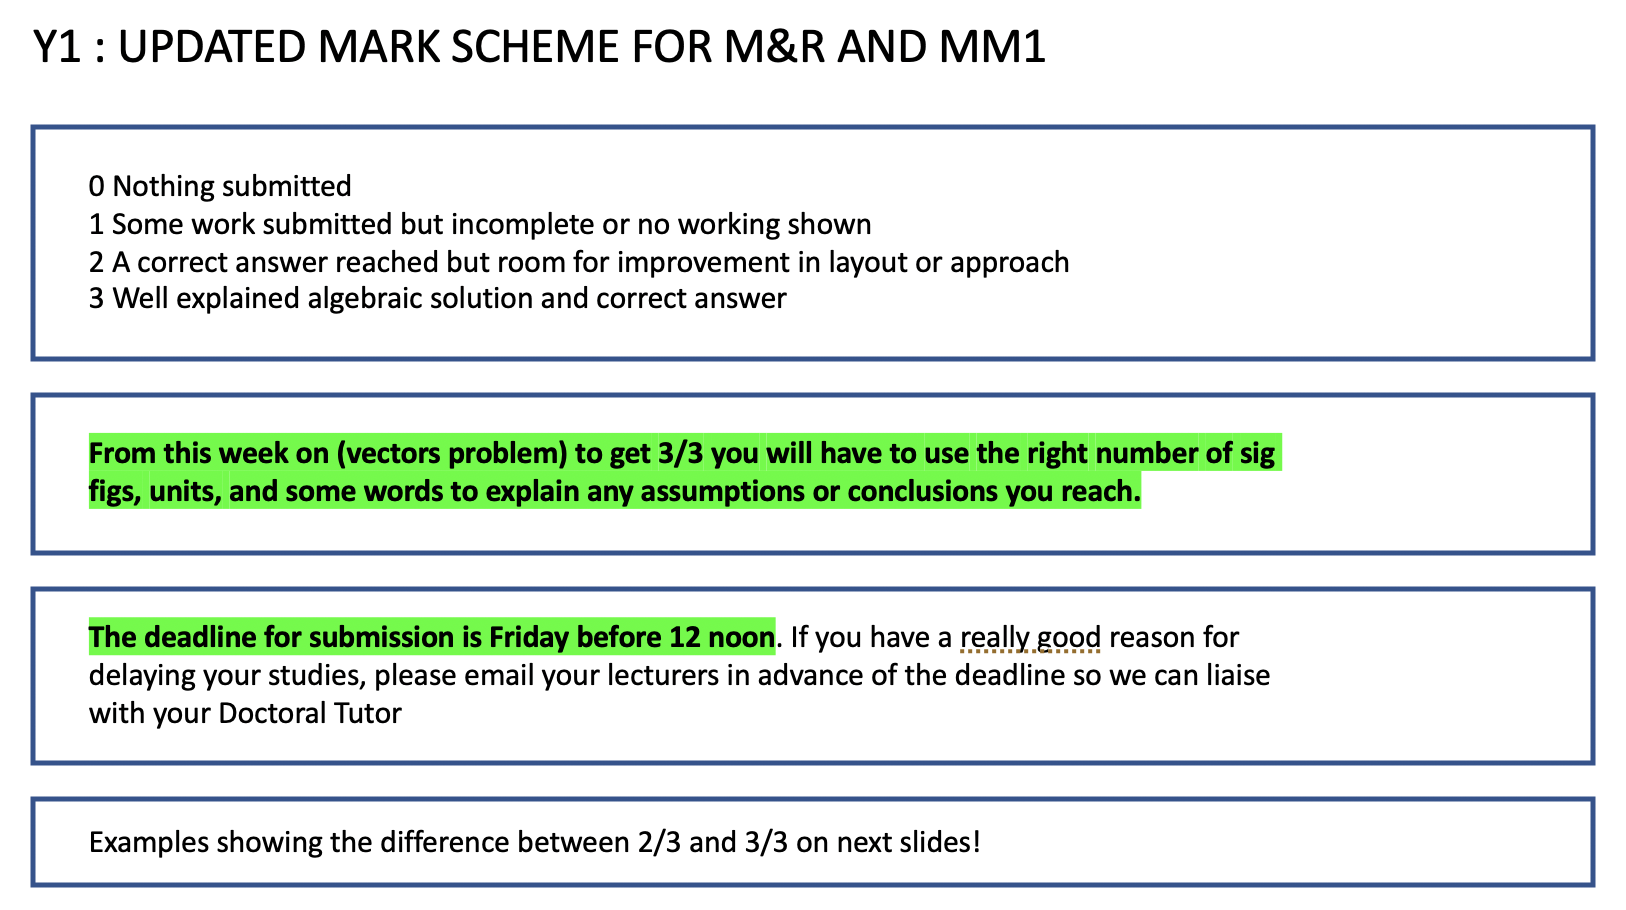
\includegraphics[scale=0.34]{markscheme}
%The workshop problems (1 per week for 10 weeks) = 10\% of your final mark\\[1ex]
\end{frame} 

\begin{frame}
\frametitle{Submit your workshop problem (vectors) for marking by noon Friday}
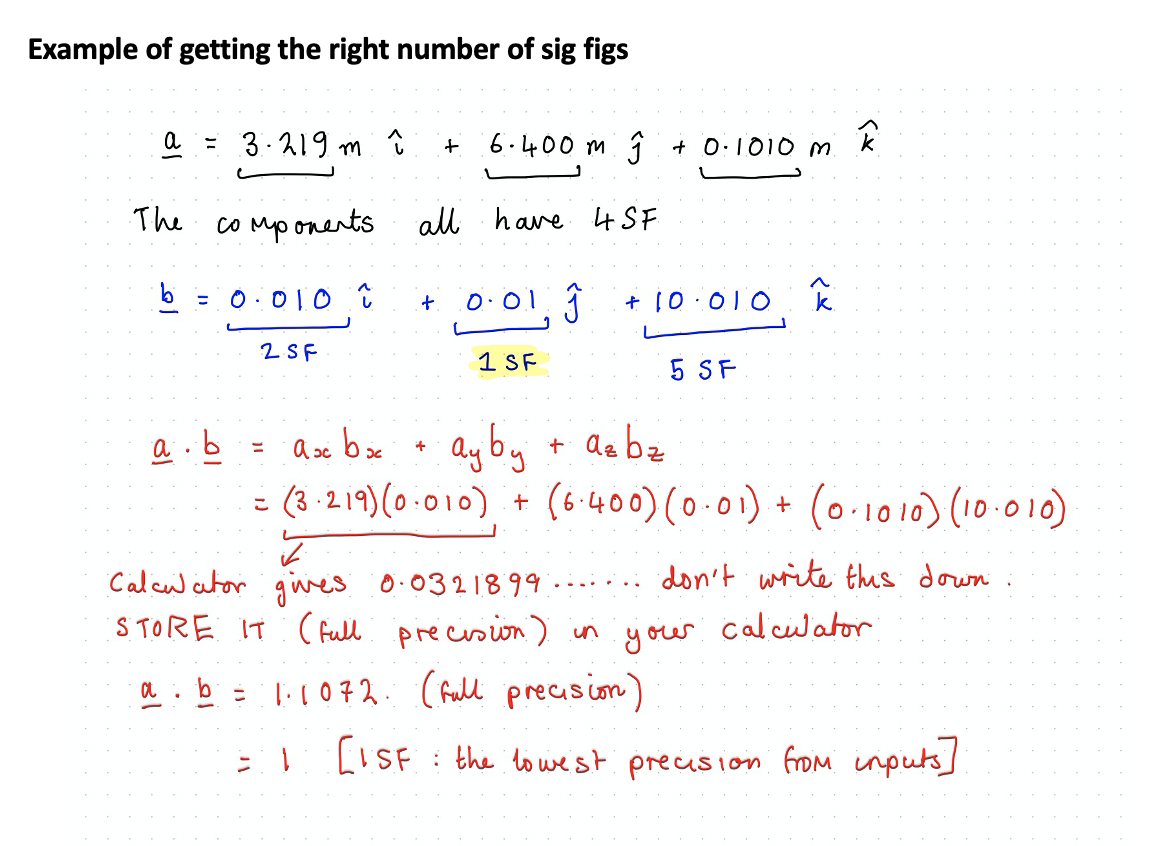
\includegraphics[scale=0.34]{sigfigs}
\end{frame} 

\begin{frame}
\frametitle{Submit your workshop problem (vectors) for marking by noon Friday}
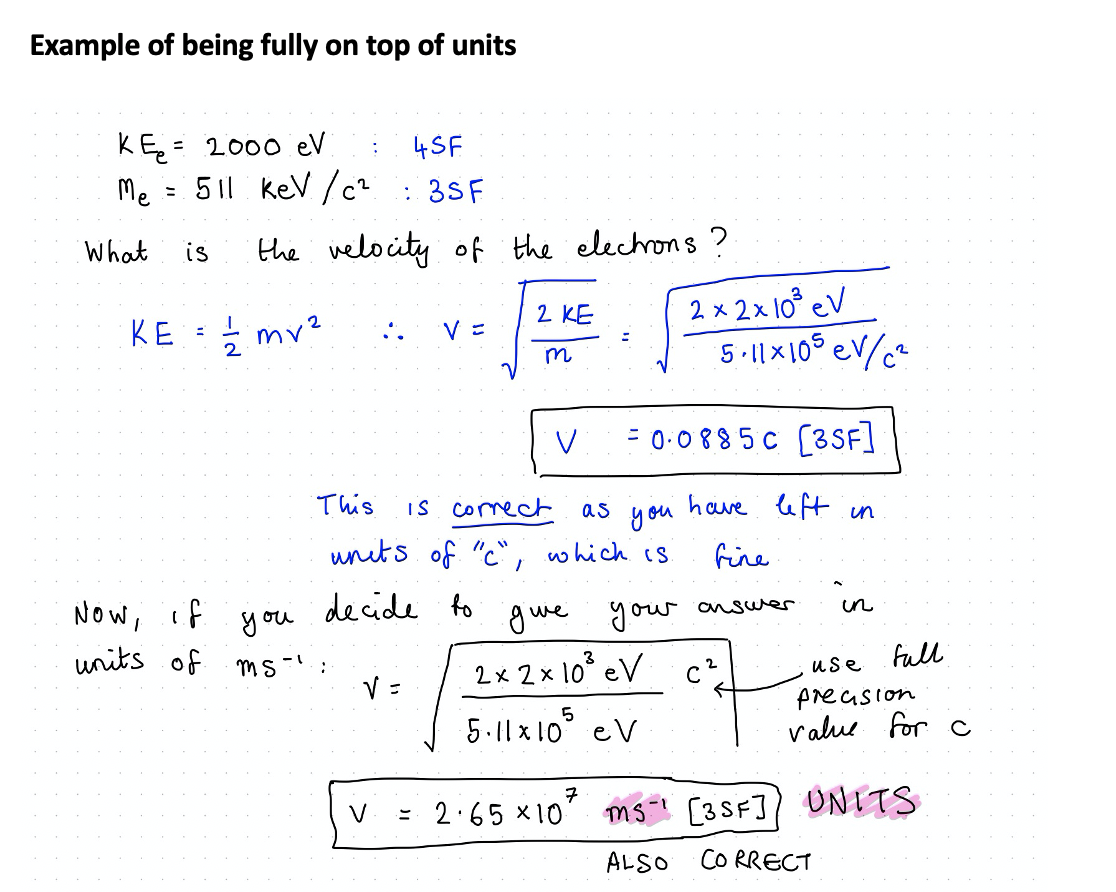
\includegraphics[scale=0.34]{units}
\end{frame} 
 %-----------------------------------------------------------%
 % 1 Kinematics                                                 %
 %-----------------------------------------------------------%
\section{M\&R 3: Motion in two and three dimensions}
\begin{frame}
\frametitle{Vectors} 
\normalsize

This week's topics:\\[3ex]

\begin{itemize}
\item[3.1] Projectiles\\[3ex]
\item[3.2] Uniform Circular Motion\\[3ex]
\item[3.3] Problem Solving\\[3ex]
\end{itemize}
\end{frame} 
 

 \subsection{Projectiles}

\begin{frame}{A problem in the vertical plane}
Projectiles are ``2D" problems; but we can split them into two ``1D" problems.\\[22ex]

\end{frame}



\begin{frame}{Projectile Motion}

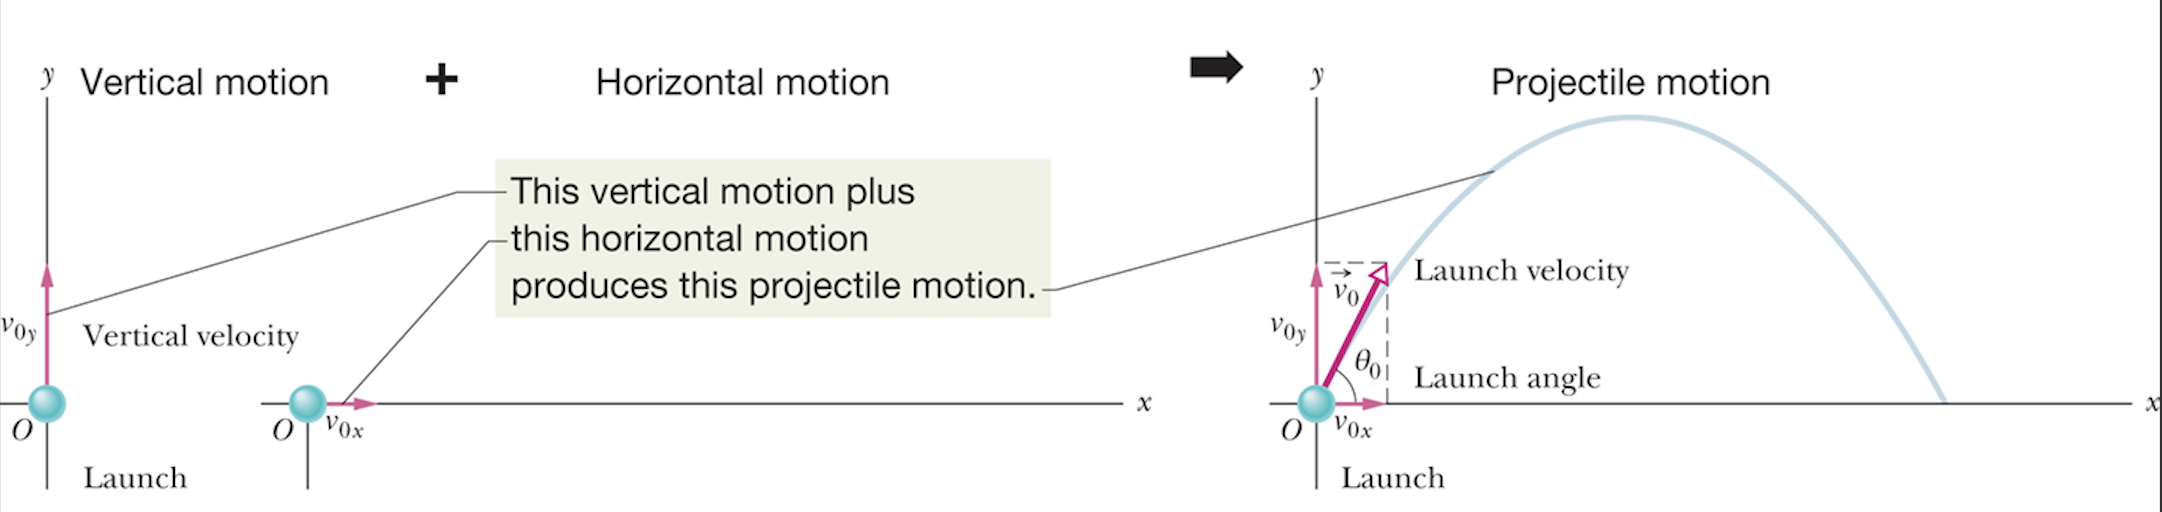
\includegraphics[scale=0.32]{proj1}

\end{frame}

\begin{frame}{Projectile Motion}

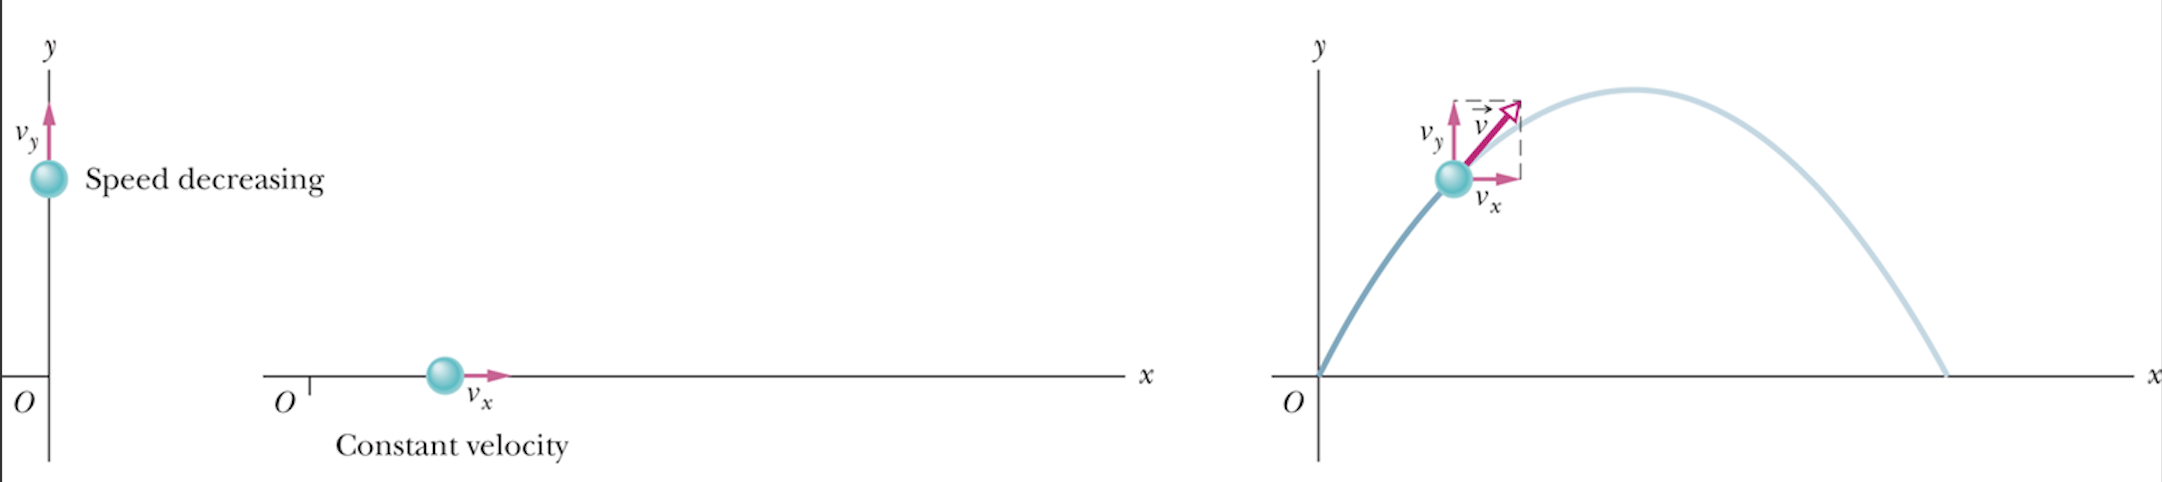
\includegraphics[scale=0.32]{proj2}

\end{frame}

\begin{frame}{Projectile Motion}

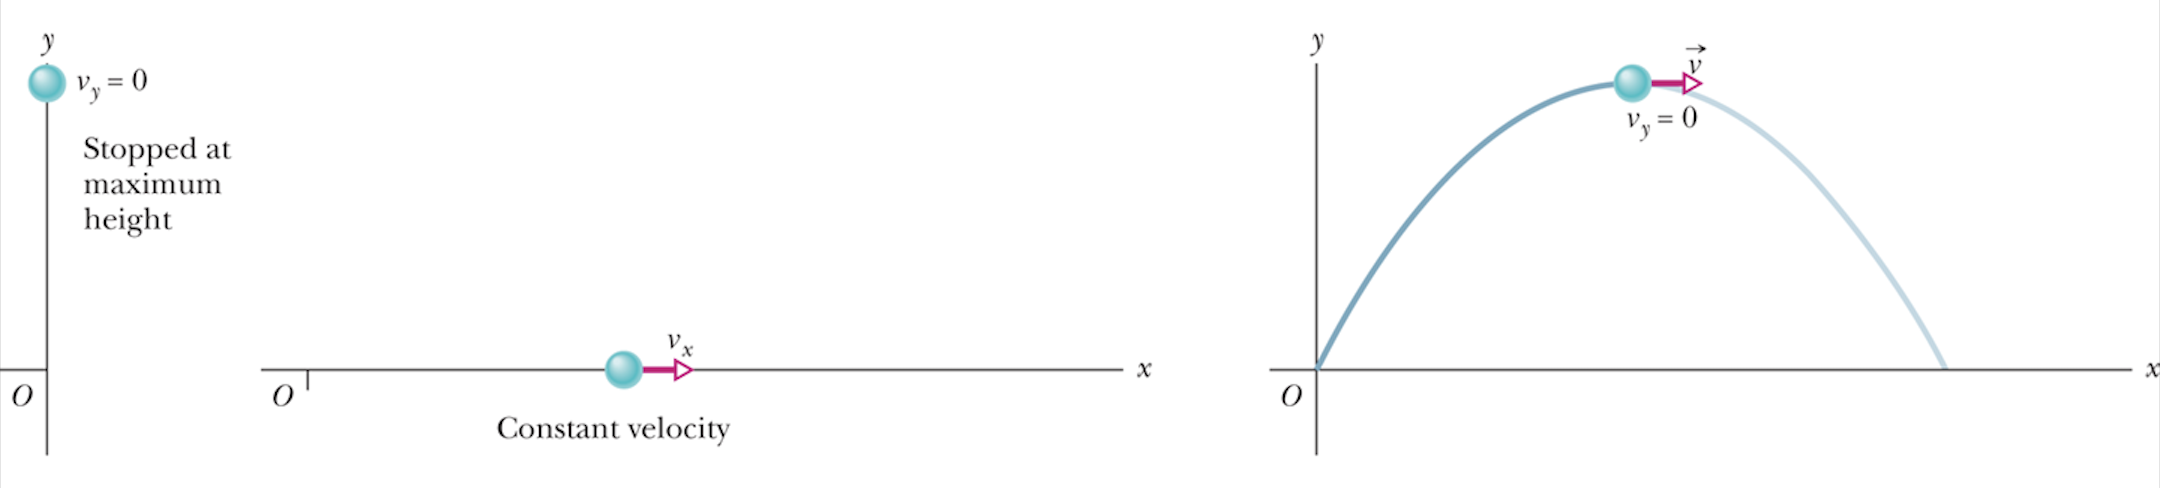
\includegraphics[scale=0.32]{proj3}

\end{frame}

\begin{frame}{Projectile Motion}

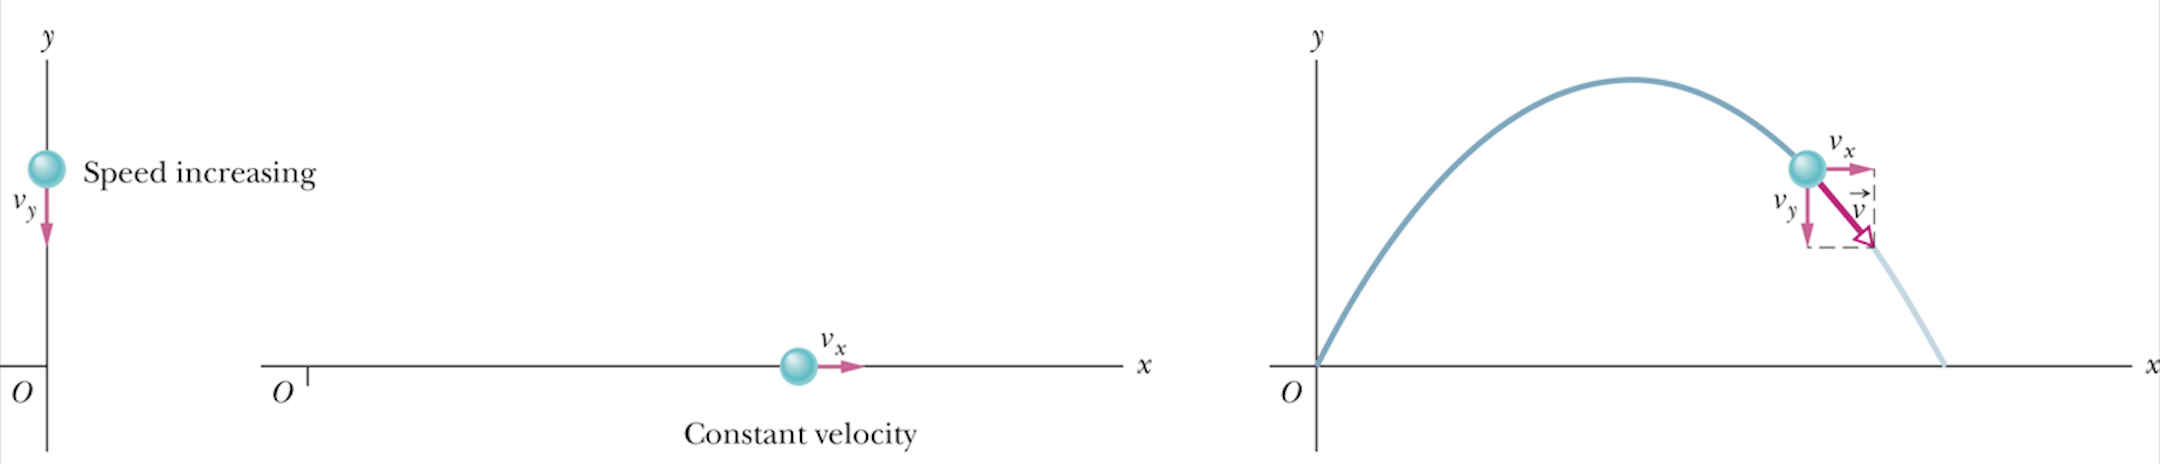
\includegraphics[scale=0.32]{proj4}

\end{frame}

\begin{frame}{Projectile Motion}

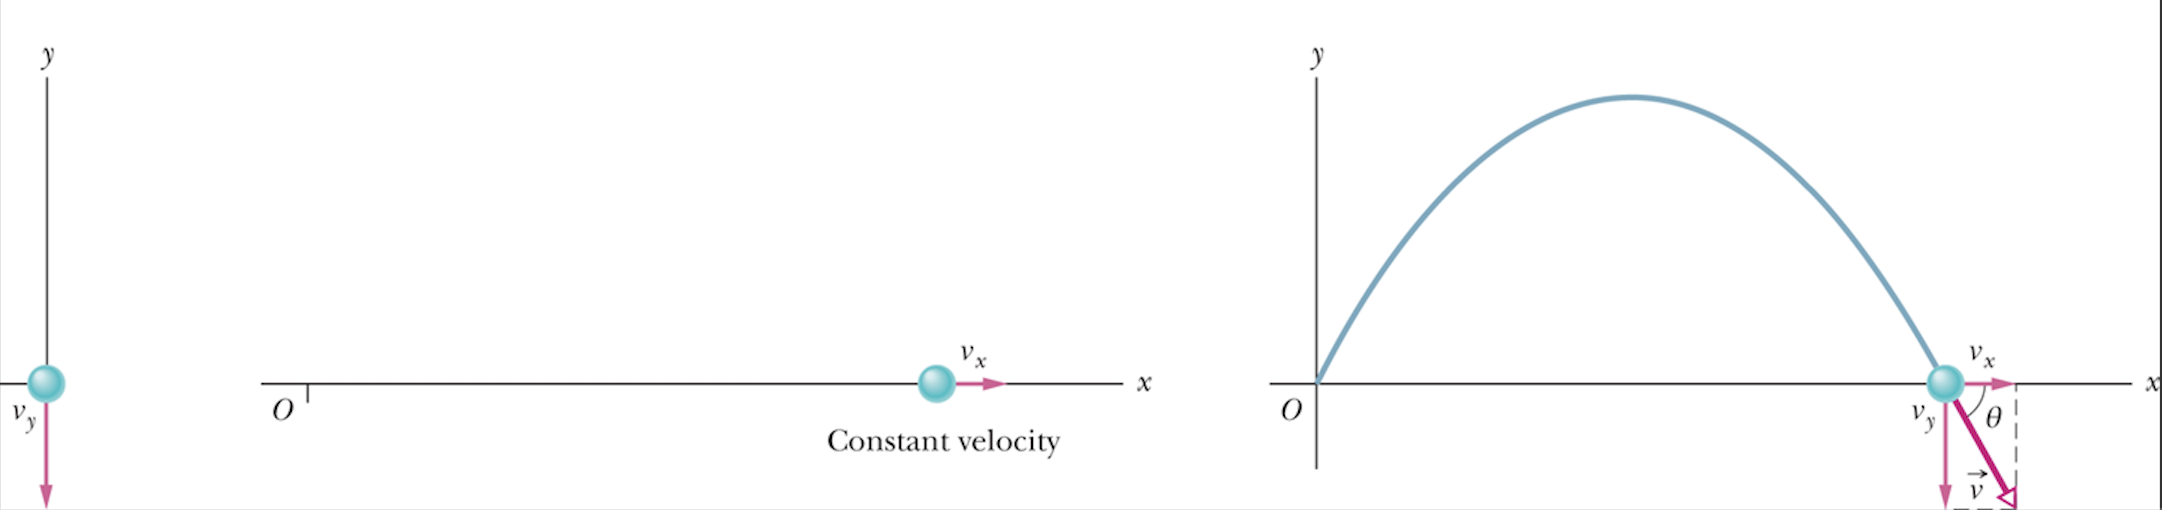
\includegraphics[scale=0.32]{proj5}

\end{frame}

\begin{frame}{Divide and Conquer}
\begin{center}
$s= ut + \frac{1}{2} at^2$ 
\end{center}



\begin{columns}
\begin{column}{0.5\textwidth}
\begin{center}
Horizontal Motion
\end{center}
\vspace{12cm}

\end{column}
\begin{column}{0.5\textwidth}
\begin{center}
Vertical Motion
\end{center}
\vspace{12cm}

\end{column}
\end{columns}
\end{frame}


\begin{frame}{Example: ball rolling off a cliff}
\small
A small ball rolls horizontally off the edge of a tabletop that is 1.20 m high. It strikes the floor at a point 1.52 m horizontally from the table edge.\\
 (a) How long is the ball in the air? \\
 (b) What is its speed at the instant it leaves the table?\\
\vspace{10cm}

\end{frame}


\begin{frame}{The Path of a Projectile}
The path is described like $y(x)$: want to eliminate $t$\\
\vspace{12cm}


\end{frame}

\begin{frame}{Horizontal Range}
At its maximum range, the vertical displacement of a projectile is zero.*
\vspace{12cm}


\end{frame}


\begin{frame}{Vertical range}
At its maximum height, the vertical speed of a projectile is zero.
\vspace{12cm}


\end{frame}



%LECTURE 2


\begin{frame}{Unpopular Adaptive Practice Problems}

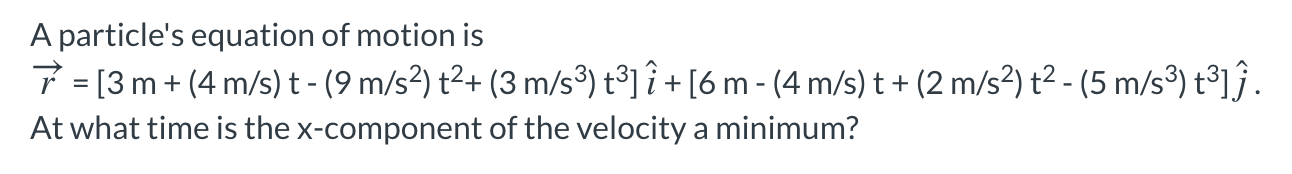
\includegraphics[scale=0.45]{minima}
\vspace{10cm}
\end{frame}


\begin{frame}{Unpopular Adaptive Practice Problems}

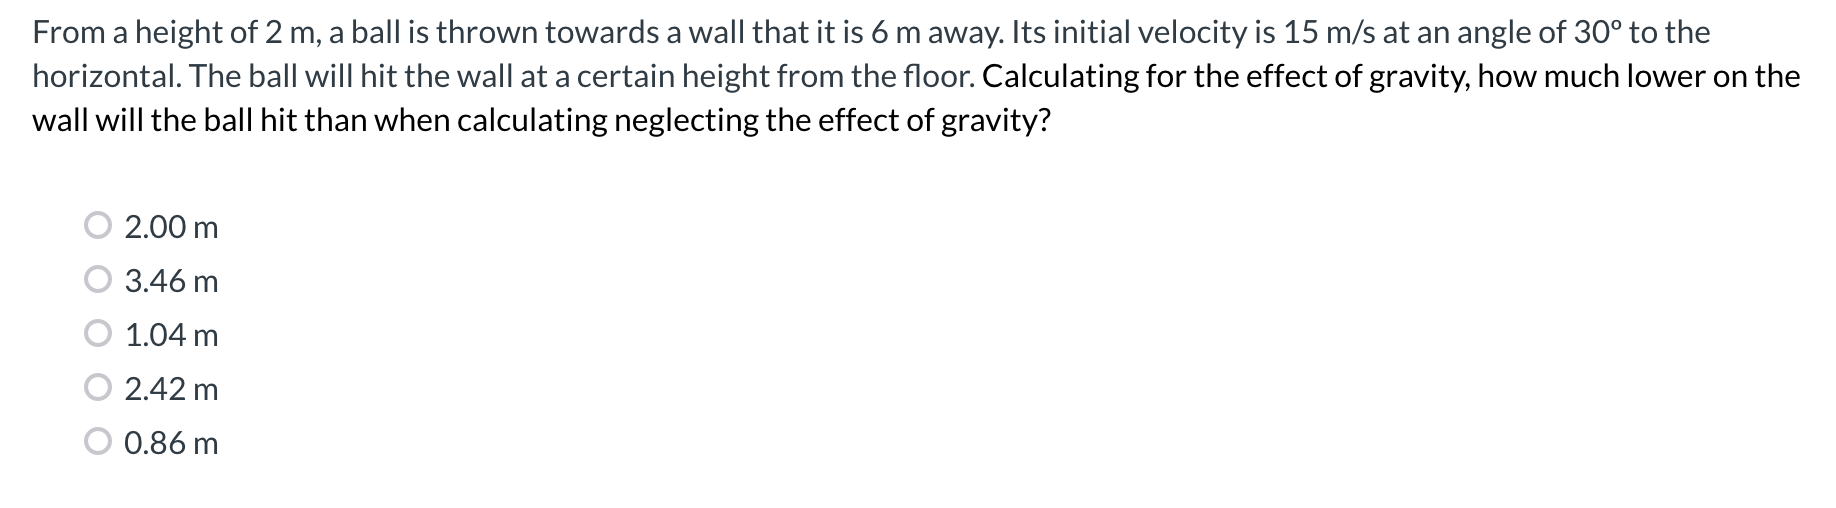
\includegraphics[scale=0.4]{ballthrow}
\vspace{10cm}
\end{frame}




 \subsection{Uniform Circular Motion}


\begin{frame}{Uniform Circular Motion}

%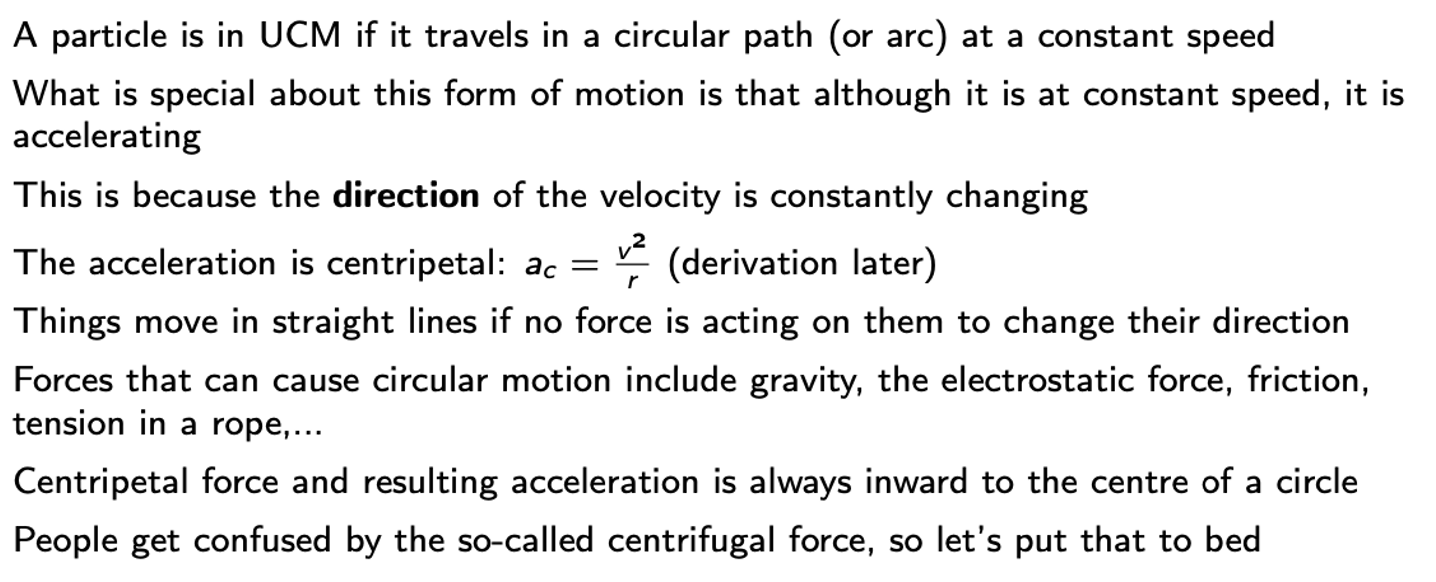
\includegraphics[scale=0.32]{ucm-intro}
\end{frame}


\begin{frame}{Some thoughts on the Centripetal Force}
Everything moves in a straight line at constant velocity, unless a force is present.\\
\vspace{20cm}


\end{frame}


\begin{frame}{Circles: $s = r\theta$}

Circumference: \\[2ex]
Radius: \\[2ex]
Angle of one full rotation: \\[2ex]
Arc length on circumference: \\[20ex]

\end{frame}

\begin{frame}{Angular Variables}



\end{frame}



\begin{frame}{The Chain Rule: $\frac{du}{dt} = \frac{du}{d\theta} \frac{d\theta}{dt} $}

The radius $r$ is constant for a circle, but the radius vector $\vect{r}$ is changing with time.\\
\vspace{20cm}

%$\frac{d}{dt} \left( \cos \theta(t) \right) = \frac{d}{dt} \left( \cos \theta \right) \frac{d\theta}{dt}  $




\end{frame}

%\begin{frame}{The Product Rule: $\frac{d}{dt} uv =  \frac{du}{dt}v + u\frac{dv}{dt} $}
%
%
%
%
%\end{frame}

\begin{frame}{Circles: $r$ is constant, but $\vect{r}$ is changing!}




\end{frame}

\begin{frame}{The Acceleration(s)}




\end{frame}

%\begin{frame}{Summary of angular variables}
%
%
%
%\end{frame}





 \subsection{Problems}
 

 \begin{frame}{Problem: plane dropping load}
\notsotiny
A rescue plane flies at  $v = 55.0$ ms$^{-1}$ and constant height $h = 500$ m toward a point directly over a victim, where a rescue capsule is to land. What should be the angle $\phi$ of the pilot's line of sight to the victim when the capsule release is made?\\
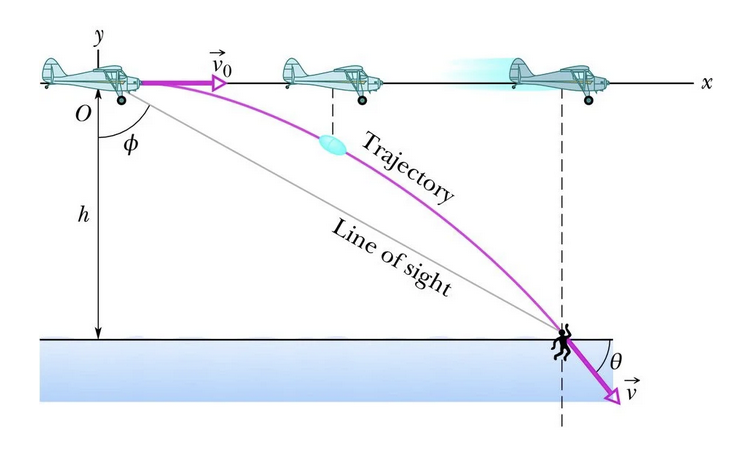
\includegraphics[scale=0.5]{planeload}
\vspace{8cm}

\end{frame}

\begin{frame}{Problem: astronaut in a centrifuge}

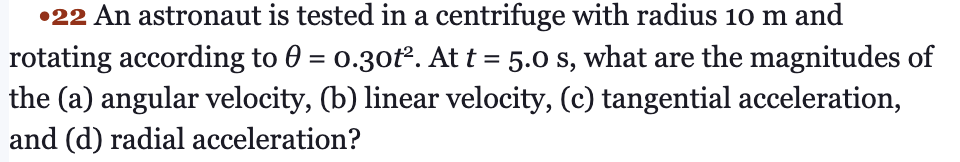
\includegraphics[scale=0.5]{astronaut}

\end{frame}


\begin{frame}{Problem: satellite in orbit}

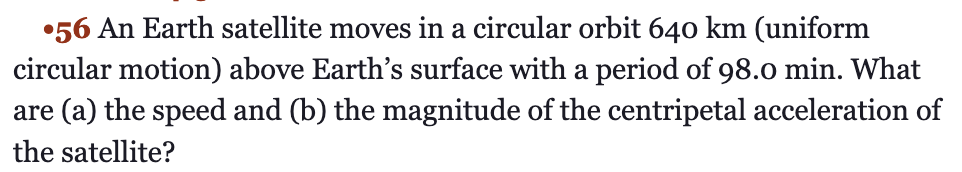
\includegraphics[scale=0.5]{satellite}

\end{frame}


\begin{frame}{Problem: killer projectile problem}
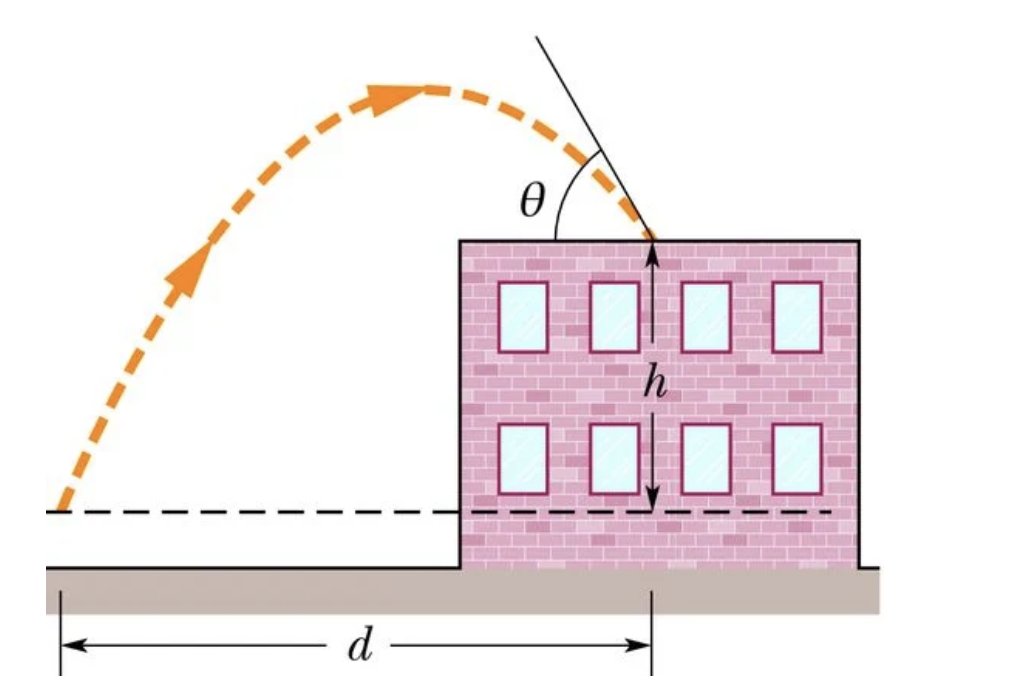
\includegraphics[scale=0.5]{killer}

\end{frame}
 
\end{document}